
% Preamble
\documentclass[12pt,a4paper]{article}

% Packages
\usepackage[utf8]{inputenc}
\usepackage[T1]{fontenc}
\usepackage{amsmath}
\usepackage{amsfonts}
\usepackage{amssymb}
\usepackage{graphicx}
\usepackage[margin=2.5cm]{geometry}
\usepackage{fancyhdr}

\usepackage{listings}          % For code snippets
\usepackage{xcolor}            % For colored text and boxes
\usepackage{tcolorbox}         % For nice looking boxes
\usepackage{enumitem}          % For better lists
\usepackage{tikz}              % For drawings and diagrams
\usepackage{mathtools}         % Enhanced math tools
\usepackage{tocloft}           % For customizing ToC
\usepackage{etoolbox}          % For patching commands
\usepackage{parskip}
\usepackage[spanish]{babel}
\usepackage{cite}
\usepackage{url}
\usepackage{hyperref}

\graphicspath{{images/}}
\bibliographystyle{unsrt}

\newcommand{\courseTitle}{Deep Learning}
\newcommand{\college}{Pontificia Universidad Católica del Perú}
\newcommand{\faculty}{Facultad de Ciencias e Ingeniería}
\newcommand{\courseCode}{1INF52}
\newcommand{\semester}{2025-0}
\newcommand{\noteDate}{\today}
\newcommand{\authors}{
    \begin{tabular}{@{}l@{\hspace{4em}}l@{}}
        Cántaro Márquez, Patricia Natividad & 20210907 \\[0.5cm]
        Nicho Manrique, Saymon Estefano & 20211866 \\[0.5cm]
        Zegarra Barrenechea, Carlos Eduardo & 20216177
    \end{tabular}
}

% for important notes
\newtcolorbox{important}[1]{
    colback=red!5!white,
    colframe=red!75!black,
    title=\textbf{#1}
}

% header and footer setup
\pagestyle{fancy}
\fancyhf{}
\rhead{\courseTitle}
\lhead{\courseCode}
\cfoot{\thepage}
\setlength{\headheight}{14.5pt}

\setlength{\parindent}{0pt}

% Document
\begin{document}

    \begin{titlepage}
    \centering
    % college
    \vspace*{0.5cm}
    {\Huge\bfseries \college \par}
    \vspace{1cm}
    {\Large\bfseries \faculty \par}
    \vspace{1cm}
    
\includegraphics[width=0.6\textwidth]{images/pucp}
    \vspace{2cm}

    % course
    {\Large\bfseries \courseTitle\ (\courseCode) \par}
    \vspace{1.5cm}
    {\large\bfseries Informe de Proyecto \par}
    \vspace{2cm}
    \authors
    \vspace{2cm}

    % date
    {\large \noteDate \par}
    \vfill
\end{titlepage}
    \tableofcontents
    \newpage
    \section{Introduction}
\label{sec:intro}

    \begin{frame}
    \frametitle{Introduction and Problem Statement}
    \begin{itemize}
        \item The increasing frequency of wildfires has led to a demand for \textbf{automated monitoring systems}.
        \item Traditional methods (satellites, thermal sensors) suffer from \textbf{delayed data retrieval}.
        \item \textbf{Deep Learning} can improve detection \textbf{speed and accuracy}.
    \end{itemize}

    \begin{figure}
        \centering
        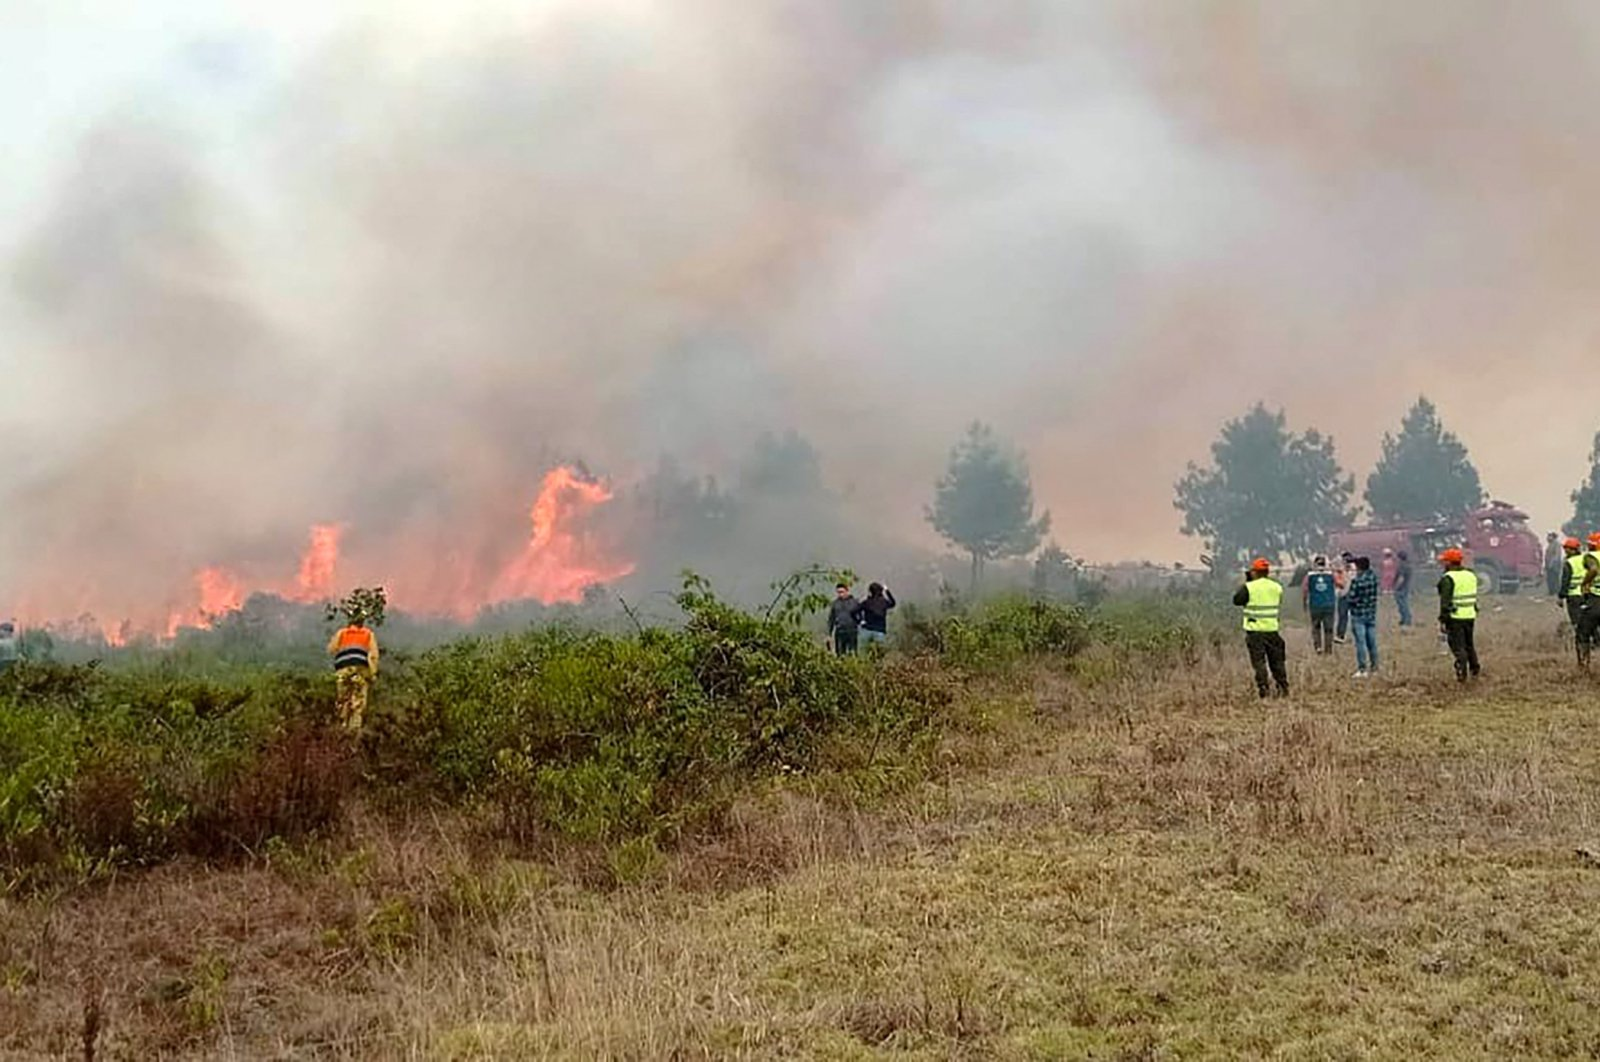
\includegraphics[width=0.4\textwidth]{images/wildfire}
        \caption{Wildfire in Peru, 2024.}\label{fig:wildfire}
    \end{figure}
\end{frame}

\begin{frame}
    \frametitle{Research Motivation and Goals}
    \blocky{Objective of this Study}{
        \begin{itemize}
            \item Develop an \textbf{ensemble of CNNs} for \textbf{wildfire detection} in aerial images.
            \item Evaluate the performance of \textbf{Xception, DenseNet121, and ResNet152}.
            \item Improve classification accuracy while keeping computational efficiency.
        \end{itemize}
    }
\end{frame}
    \section{Problem Statement}
\label{sec:problem-statement}

Although deep learning has led to remarkable progress in wildfire detection, many existing
architectures remain too large or computationally expensive to deploy on a drone.
This limits their practicality in real-time aerial monitoring.

Additionally, although there exist optimized models for devices with limited computational
capabilities, many have not been updated with the latest detection architectures, possibly
affecting both accuracy and speed.

Hence, our objective is to explore models that strike a balance between precision and
efficiency, enabling effective deployment on drones for early wildfire detection.

    \section{Estado del Arte}

\subsection{Métodos Clásicos y Sensores}
Existen diversos enfoques convencionales de detección de incendios:
\begin{enumerate}
    \item Sistemas basados en sensores (ópticos, de humo, de gas, de temperatura, etc)
    que pueden percibir señales asociadas al fuego, pero cuyo alcance y capacidad de
    respuesta pueden resultar limitados.
    \item Técnicas de visión clásica basadas en la segmentación de color característico
    del fuego (naranja, amarillo, rojo) o el humo (blanco, gris, negro) que han sido
    útiles en sistemas de videovigilancia tempranos, pero que suelen verse
    afectados por altas tasas de falsas alarmas (reflejos, luces parásitas, nubes con
    tonos similares, etc).
\end{enumerate}

\subsection{Métodos con ML y DL}
Con la expansión de la videovigilancia y la aparición de la visión por computadora,
se han intentado proponer métodos más sofisticados que no solo integran lo mencionado
anteriormente, sino que también agregan forma, textura, dinámica y variación de luz
para identificar el comportamiento propio del fuego.

\subsubsection{Clasificación con CNNs pre entrenadas}
Diversas arquitecturas de redes neuronales convolucionales (CNN), como pueden ser Inception,
VGGNet, Xception, DenseNet o ResNet, han demostrado resultados prometedores en la
clasificación de imágenes de fuego y humo. Sin embargo, uno de los retos es la
disponibilidad de grandes volúmenes de datos. Por ello, se han considerado diversas técnicas
que permitan sobrellevar este problema.

\begin{enumerate}
    \item \textbf{Transfer Learning:} Consiste en reutilizar una red preentrenada en un
    conjunto de datos grande y ajustarla a un conjunto de datos más pequeño y específico.
    \item \textbf{Fine Tuning:} Consiste en ajustar los pesos de una red preentrenada
    en un conjunto de datos similar al de interés, pero con una tarea diferente.
    \item \textbf{Data Augmentation:} Consiste en generar nuevas imágenes a partir de
    las existentes, aplicando transformaciones como rotaciones, traslaciones, zooms,
    cambios de brillo y contraste, etc.
\end{enumerate}

\subsubsection{Detección de objetos con YOLO}
A pesar de que las CNNs clásicas son efectivas en la clasificación de imágenes, no
son tan eficientes en la detección de objetos. Por ello, se han propuesto arquitecturas
como YOLO (You Only Look Once) que permiten identificar y localizar elementos en
imágenes en tiempo real y con alta precisión.

\subsubsection{Clasificación con Transformadores de Visión (ViTs)}
Los Vision Transformers (ViTs) han surgido como una alternativa prometedora a las
CNNs para la clasificación de imágenes. A diferencia de las CNNs,
que utilizan convoluciones para extraer características, los ViTs emplean
mecanismos de autoatención para capturar relaciones globales en la imagen.
Esta capacidad les permite modelar dependencias a largo alcance y adaptarse mejor
a variaciones en la textura y el contexto del fuego y el humo. Aunque requieren
grandes volúmenes de datos para un entrenamiento efectivo, el preentrenamiento en datasets
masivos y fine-tuning ha permitido su aplicación en la detección de incendios con
resultados competitivos.

\subsection{Hallazgos recientes destacados}

\subsubsection{Yang (2019), Mao et al. (2018)}
Desarrollaron un pipeline para clasificación de incendios forestales con CNNs pre entrenadas
de 3 modelos destacables, VGG16, InceptionV3 y Xception. Exploraron el fine tuning y usaron
optimización bayesianda con LwF. Esto demostró una mejor abrupta en los nuevos datosy
demostró el gran potencial existente en las técnicas de deep learning y transfer learning
para la detección de incendios y clasificación de imágenes.

\subsubsection{Chetoui \& Akhloufi (2024)}
Los autores propusieron emplear los modelos YOLOv8 y YOLOv7 para la detección de incendios
forestales. Para ello, usaron un dataset de 11,000 imágenes de incendios. Además, aplicaron
técnicas de fine tuning y data augmentation para mejorar el rendimiento de los modelos.
Condujeron sus experimentos en un NVidia V100SXM2 (16GB) y en un CPU Intel Gold 6148 Skylake
(2.4 GHz). Los resultados mostraron que YOLOv8 superó a YOLOv7 en términos de precisión y
recall. Incluso en situaciones con bajo contraste del humo en las imágenes de validación,
logró obtener una confianza de aproximadamente 0.8 \cite{fire7040135}.

\subsubsection{Mehta \& Rastegari (2022)}
Los autores propusieron MobileViT, un modelo ligero basado en Vision Transformers (ViTs)
optimizado para tareas de visión en dispositivos con recursos limitados, como teléfonos y
drones. A diferencia de ViTs tradicionales, que requieren una gran cantidad de parámetros y
capacidad computacional, MobileViT combina convoluciones con autoatención global para
capturar tanto características locales como globales con menos cómputo. Sus experimentos en
ImageNet-1k y MS-COCO demostraron que MobileViT supera a CNNs ligeras como MobileNetV3 y a
modelos ViT compactos como DeIT, logrando un mejor equilibrio entre precisión y eficiencia.
Este enfoque sugiere que los transformers pueden ser una opción viable para la detección
de incendios en tiempo real en drones sin comprometer rendimiento ni consumo
energético \cite{mobilevit2022}.

\subsubsection{Palaparthi \& Nangi (2023)}
Los autores desarrollaron FireSight, un modelo de clasificación de incendios basado
en imágenes aéreas capturadas por drones. Para mejorar la precisión y eficiencia en
dispositivos con recursos limitados, combinaron Vision Transformers (ViTs) con CNNs
en un modelo ensemblado. Su enfoque incluyó técnicas de fine-tuning, data augmentation
y reducción de parámetros mediante la poda de capas del ViT. Compararon su método con
arquitecturas previas como Xception y ResNet, logrando un 82.28\% de precisión en la
detección de incendios en el conjunto de datos FLAME. Sus experimentos demostraron que
el ensemblado de ViTs y CNNs captura mejor las características de fuego y humo, lo que
hace que este enfoque sea prometedor para la detección temprana de
incendios con drones \cite{firesight2023}.




    \section{Theoretical Framework}
\label{sec:theoretical-framework}

The purpose of this theoretical framework is to introduce the key concepts that allow us
to address the problem of wildfire detection using image analysis with \textit{deep
learning} techniques.
We will explore the capabilities of neural networks, specifically convolutional neural networks (CNN),
as tools for the detection and mitigation of these events.

\subsection{Convolutional Neural Networks}
\label{subsec:cnn}

Convolutional neural networks (CNNs) are a type of deep learning architecture highly
effective for processing data that can be represented as a grid, such as images.
Their design allows them to automatically learn spatial hierarchies and relevant patterns,
making them ideal for image classification and object detection tasks.

Their architecture generally consists of three main types of layers: convolutional layers,
pooling layers, and fully connected layers.
Convolutional layers apply filters to the input image to extract relevant features,
while pooling layers reduce the dimensionality of the extracted features.
Finally, fully connected layers handle the final classification, ensuring each output neuron
is connected to all neurons in the previous layer.

Using CNNs for smoke detection in wildfires has become crucial thanks to their capacity
to process large volumes of visual data, such as satellite images and surveillance camera
feeds.
This allows differentiating smoke from elements like clouds or fog, and does so
more efficiently than traditional methods.

\subsection{Xception (Extreme Inception)}
\label{subsec:xception}

Xception is an architecture based on Inception that replaces standard convolutions with
\textit{depthwise separable convolutions}, reducing the number of parameters without
affecting performance.
It splits the feature extraction into two stages: first, it filters
by channel and then mixes information across channels.
This enables more efficient learning and has shown better performance than
InceptionV3 on large datasets, although its implementation can be more computationally expensive in some cases
\cite{sathishkumar_forest_2023}.

\subsection{DenseNet}
\label{subsec:densenet}

DenseNet optimizes the flow of information by connecting each layer to all previous ones,
promoting feature reuse and improving gradient propagation.
Thanks to this structure, it manages to reduce the number of parameters compared to other deep architectures without
losing accuracy.
It is useful for very deep models, but its large number of connections can increase memory consumption during training.

\subsection{ResNet}
\label{subsec:resnet}

ResNet introduces \textit{skip connections} or residual connections that allow gradients
to pass through several layers without vanishing, solving the vanishing gradient problem
in deep networks.
Instead of learning complete transformations, it learns the differences between the input
and the expected output, making training easier and allowing networks with hundreds of layers.
Although it is highly efficient, deeper versions may require careful tuning of hyperparameters
to avoid excessive computational overhead \cite{sathishkumar_forest_2023}.

\subsection{YOLO}
\label{subsec:yolo}

You Only Look Once is an advanced object detection model designed to identify and locate
elements in images in real time with high accuracy.
Its operation is based on convolutional neural networks (CNNs) to analyze images
with a single forward pass, dividing them into grids and predicting the position,
dimensions, and class of the detected objects \cite{yaseen2024yolov8indepthexplorationinternal}.

YOLOv8, the latest version, introduces an \textit{anchor-free} approach, removing the
predefined bounding box positions used in previous versions.
This helps simplify training and improve accuracy in detecting objects of varying shapes and sizes.
It also incorporates CSPNet (\textit{Cross-Stage Partial Networks}) as a backbone, an architecture that optimizes
the flow of information and reuses features from earlier layers to reduce redundancies
and improve computational efficiency.

These characteristics make YOLOv8 highly effective for real-time tasks and for surveillance
and environmental monitoring, such as wildfire detection \cite{s23208374}.

\subsection{Transfer Learning}
\label{subsec:transfer-learning}

Transfer learning is a machine learning technique that involves reusing knowledge learned
in one domain to improve performance in another related domain.
In the context of neural networks, this involves taking a network pretrained on a large dataset and adapting it
to a smaller, more specific dataset.

    \section{State of the Art and Baseline}
\label{sec:baseline}

\begin{frame}
    \frametitle{Traditional Approaches to Wildfire Detection}
    \begin{itemize}
        \item \textbf{Sensor-based methods:} Use \textbf{temperature, smoke, and gas sensors}, but have \textbf{limited coverage}.
        \item \textbf{Classic Computer Vision methods:} Use \textbf{color-based segmentation}, but suffer from \textbf{high false positives}.
        \item \textbf{Machine Learning and Deep Learning approaches:}
            \begin{itemize}
                \item CNN-based classification (e.g., Xception, DenseNet, ResNet).
                \item Object detection with \textbf{YOLOv8}.
                \item Vision Transformers (\textbf{ViTs}) for feature extraction.
            \end{itemize}
    \end{itemize}
\end{frame}

\begin{frame}
    \frametitle{Baseline Model: FireSight (Stanford)}
    \begin{itemize}
        \item FireSight combines \textbf{CNNs and ViTs} for aerial wildfire detection.
        \item Achieves \textbf{82.28\% accuracy} using \textbf{DenseNet + ResNet + ViT} ensemble.
        \item Our approach:
            \begin{itemize}
                \item Improve CNN-only ensemble.
                \item Optimize architecture for \textbf{real-time drone deployment}.
            \end{itemize}
    \end{itemize}
\end{frame}
    \section{Propuesta de Modelo}

\subsection{Dataset}
Se usará el FLAME dataset \cite{FLAME_Dataset} ya que este ha sido diseñado para estudios de
detección y segmentación de incendios, conteniendo imágenes y videos capturados mediante
drones en bosques del norte de Arizona. Para este proyecto, se usarán solo las imágenes y
se aprovechará que estas ya han sido distribuidas y etiquetadas para ser usadas:
39,375 imágenes para entrenamiento/validación y 8,617 imágenes para testeo.

\subsection{Arquitectura Propuesta}
Con el dataset de FLAME, se usará un ensamble de 3 modelos, los cuales serán: Xception,
DenseNet y ResNet; y posteriormente se destilarán en un modelo ligero como lo es
MobileNetV3. Además, se usarán ténicas de pruning antes del deployment para reducir
el tamaño del modelo y mejorar la eficiencia en la inferencia.

\begin{figure}[h]
    \centering
    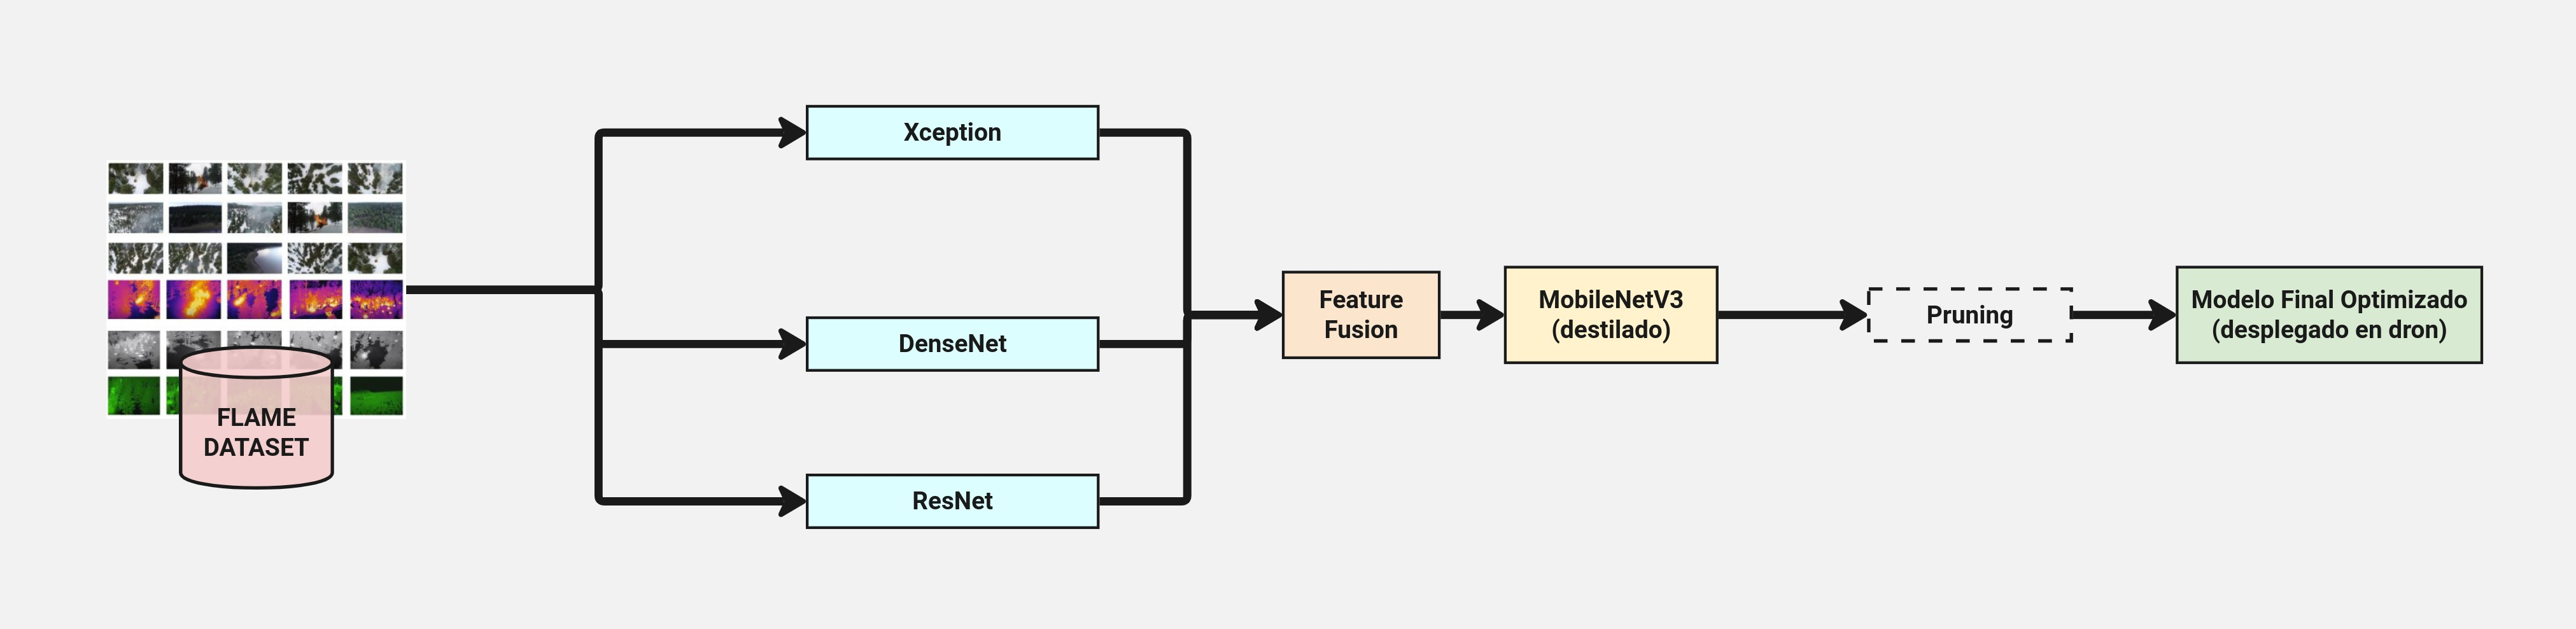
\includegraphics[width=0.9\textwidth]{images/model}
    \caption{Descripción del modelo}
    \label{fig:model}
\end{figure}

Se utilizarán \textbf{CNNs entrenadas sobre el dataset FLAME}, específicamente:

\begin{itemize}
    \item \textbf{Xception}: Utiliza \textit{Depthwise Separable Convolutions (DSC)} para optimizar la extracción de características, capturando relaciones complejas en la imagen. Se considera más eficiente en comparación con arquitecturas tradicionales.
    \item \textbf{DenseNet}: Usa \textit{bloques densos} que facilitan la reutilización de características, beneficiando la detección de elementos sutiles como \textit{ríos o humo de bajo contraste}.
    \item \textbf{ResNet}: Implementa \textit{conexiones residuales} para evitar la degradación del gradiente en redes profundas, lo que mejora la convergencia en entrenamientos largos.
\end{itemize}

\subsubsection{Entrenamiento previo al ensamble}
Cada modelo se entrenará \textbf{de manera individual} para la clasificación de incendios, empleando \textit{cross-entropy} como función de pérdida y aplicando \textit{early stopping} para evitar el sobreajuste.

\subsubsection{Fusión de Modelos (Ensamble)}
Una vez completados los entrenamientos individuales, se procederá con la fusión de modelos. Se consideran dos estrategias:

\begin{enumerate}
    \item \textbf{Fusión a nivel de salidas finales}:
    \begin{itemize}
        \item Se combinan las \textit{probabilidades} generadas por los tres modelos en un vector mayor.
        \item Se ajusta el \textit{peso} de cada modelo y se valida con \textit{cross-validation}.
    \end{itemize}

    \item \textbf{Fusión en capas intermedias}:
    \begin{itemize}
        \item Se extraen \textit{vectores de características} desde capas intermedias de cada modelo y se concatenan en un vector mayor.
        \item Se entrena un \textit{clasificador adicional} sobre este vector fusionado para generar la salida final.
    \end{itemize}
\end{enumerate}

\subsubsection{Knowledge Distillation}
Dado que el ensamble es \textbf{demasiado grande} para dispositivos con recursos limitados, se aplicará \textit{Knowledge Distillation}. Se entrenará un \textbf{MobileNetV3} como versión comprimida del ensamble, preservando la mayor cantidad de información relevante.

\subsubsection{Optimización Adicional: Pruning}
Para reducir aún más el tamaño del modelo, se aplicará \textit{pruning}, eliminando \textbf{pesos irrelevantes o de magnitud baja}. Esto permite reducir la carga computacional sin afectar significativamente la precisión.

\subsection{Justificación}

\begin{itemize}
    \item \textbf{Uso de Xception, DenseNet y ResNet en paralelo:}
    \begin{itemize}
        \item \textbf{Xception}: Usa convoluciones separables, reduciendo cálculos sin perder precisión.
        \item \textbf{DenseNet}: Mejora reutilización de características, ideal para detectar detalles pequeños.
        \item \textbf{ResNet}: Usa conexiones residuales, facilitando el entrenamiento en redes profundas.
    \end{itemize}
    \item \textbf{Destilación en MobileNetV3:}
    \begin{itemize}
        \item Modelo ligero y eficiente para \textit{drones}.
        \item Mantiene precisión al aprender de los modelos grandes.
    \end{itemize}
    \item \textbf{Ventajas sobre el estado del arte:}
    \begin{itemize}
        \item Más eficiente que ViT y ResNet en inferencia en dispositivos de bajo consumo.
        \item Mejor precisión que modelos CNN individuales.
    \end{itemize}
    \item \textbf{Despliegue en \textit{drones}:}
    \begin{itemize}
        \item Menor consumo de energía que ViT y CNNs pesados.
        \item Inferencia en tiempo real en \textit{Jetson Nano, Coral TPU, Raspberry Pi}.
    \end{itemize}
<<<<<<< HEAD
\end{itemize}
=======
\end{itemize}

\subsection{Pipeline}
El flujo de producción está diseñado para ejecutar una secuencia de cinco pasos que garantizan reproducibilidad y eficiencia. Estos pasos son:

\begin{enumerate}
    \item \textbf{Entrenamiento de DenseNet:} El modelo DenseNet se entrena utilizando hiperparámetros fijos y ajustados.
    \item \textbf{Entrenamiento de ResNet:} De manera similar, el modelo ResNet se entrena con sus mejores hiperparámetros.
    \item \textbf{Entrenamiento de Xception:} El modelo Xception se entrena bajo el mismo enfoque.
    \item \textbf{Ensamblado de modelos:} Las predicciones de los tres modelos entrenados se promedian para construir un modelo en ensamblado.
    \item \textbf{Destilación del modelo:} El modelo ensamblado actúa como maestro para destilar el conocimiento en un modelo estudiante más ligero.
\end{enumerate}

El script de bash (ubicado en \texttt{scripts/run\_pipeline.sh}) orquesta el flujo de trabajo.
>>>>>>> ae2c2836c37fe2e4b4ffbc943703ef797c84c406

    \section{Data Preprocessing}
\label{sec:data-preprocessing}

In this section, we describe our approach to preparing the FLAME dataset before training.
Since the dataset is already structured for the wildfire classification task, \textbf{no data augmentation was applied}.
We focused on analyzing the dataset distribution and ensuring the images were properly formatted for training.

\subsection{Data Distribution}
\label{subsec:data-distribution}

We examined the distribution of images across the two categories: \textit{Fire} and \textit{No\_Fire}.
The \textbf{training set} contains \textbf{63.55\% Fire} images (25,027) and \textbf{36.45\% No\_Fire} images (14,357).
The \textbf{test set} consists of \textbf{3,480 Fire} images and \textbf{5,137 No\_Fire} images.

All images were resized to \textbf{224\(\times\)224} pixels to maintain consistency across model inputs.
Additionally, pixel values were normalized to the \textbf{[0,1]} range before being fed into the model.


    \section{Entrenamiento}
En esta sección, describimos la primera fase de nuestro experimento con la arquitectura
DenseNet. El objetivo de este entrenamiento inicial es obtener un modelo base
y analizar aspectos clave como la estabilidad de la pérdida, el sobreajuste
y los desbalances en las clases. Los resultados de esta fase servirán como base para
mejorar el modelo y el entrenamiento de los demás en las siguientes iteraciones.


\subsection{Hiperparámetros}
\subsubsection{Tamaño del Batch (Batch Size)}
\begin{itemize}
    \item \textbf{Inicial:} 16
    \item \textbf{Optimización:} Se redujo a 8 en la última versión del modelo para mejorar la \textbf{generalización}, reduciendo la probabilidad de sobreajuste.
\end{itemize}

\subsubsection{Tasa de Aprendizaje (Learning Rate)}
\begin{itemize}
    \item \textbf{Inicial:} 0.001
    \item \textbf{Optimización:} Se redujo a 0.0001 para hacer los ajustes de los pesos más suaves y evitar grandes oscilaciones en la pérdida.
\end{itemize}

\subsubsection{Optimizador}
\begin{itemize}
    \item \textbf{Inicial:} Adam
    \item \textbf{Optimización:} Se mantuvo Adam porque ofrece una actualización eficiente de los pesos con momentums adaptativos, pero se ajustaron sus hiperparámetros internos.
\end{itemize}

\subsubsection{Fine-Tuning)}
\begin{itemize}
    \item \textbf{Modelo 2:} Se descongelaron 10 capas de DenseNet, pero esto no mejoró la precisión.
    \item \textbf{Modelo 3:} Se redujo a 5 capas, logrando un entrenamiento más estable sin tanto sobreajuste.
\end{itemize}

\subsubsection{Loss Function}
\begin{itemize}
    \item \textbf{Inicial:} Cross-Entropy estándar.
    \item \textbf{Optimización:} Se agregó \textbf{pesado de clases (class weighting)} para reducir el sesgo del modelo hacia imágenes de "Fuego" y mejorar la detección de "No Fuego".
\end{itemize}

\subsubsection{Balanceo de Clases}
\begin{itemize}
    \item \textbf{Problema:} El dataset tenía muchas más imágenes de "Fuego" que de "No Fuego".
    \item \textbf{Solución:} Se aplicó pesado de clases en la función de pérdida, obligando al modelo a prestar más atención a la clase minoritaria.
\end{itemize}

\subsubsection{Epochs}
\begin{itemize}
    \item \textbf{Inicial:} 30 épocas.
    \item \textbf{Optimización:} Se ha mantenido, pero con ajustes en la tasa de aprendizaje y el batch size para evitar sobreajuste prematuro.
\end{itemize}

\subsubsection{Data Augmentation}
\begin{itemize}
    \item \textbf{Inicial:} Transformaciones básicas como escalado y normalización.
    \item \textbf{Optimización:} Se añadieron rotaciones, flips horizontales y cambios de brillo y contraste para mejorar la robustez del modelo.
\end{itemize}

\subsubsection{Early Stopping}
\begin{itemize}
    \item Habilitado para detener el entrenamiento si la pérdida de validación deja de mejorar después de un cierto número de épocas, evitando un uso innecesario de recursos.
\end{itemize}

\subsubsection{Número de Neuronas en Capas Densas}
\begin{itemize}
    \item \textbf{Denso Final:} Se mantuvo en 512 neuronas con activación ReLU antes de la capa de salida.
\end{itemize}

\paragraph{Regularización L2}
\begin{itemize}
    \item Añadida en las capas densas para evitar sobreajuste al penalizar valores de pesos muy altos.
\end{itemize}

\subsubsection{Dropout}
\begin{itemize}
    \item \textbf{Inicial:} 0.3
    \item \textbf{Optimización:} Aumentado a 0.5 en la última versión para mejorar la robustez del modelo reduciendo la dependencia de neuronas individuales.
\end{itemize}

\subsubsection{Análisis de Mejoras del Modelo}

\paragraph{Modelo 1 $\rightarrow$ Modelo 2}
\begin{itemize}
    \item El ajuste fino (descongelar 10 capas) no mejoró la precisión.
    \item La pérdida de validación disminuyó, pero el sobreajuste aumentó.
    \item El desbalance de clases siguió siendo un problema grave (Recall de "No Fuego" = 0.02).
    \item El modelo tenía un sesgo fuerte hacia las imágenes de "Fuego".
\end{itemize}

\subsubsection{Modelo 2 $\rightarrow$ Modelo 3}
\begin{itemize}
    \item Se redujo el ajuste fino de 10 capas a 5 capas $\rightarrow$ Mayor estabilidad.
    \item La pérdida de validación se volvió más estable.
    \item El Recall de "No Fuego" mejoró de 0.02 a 0.06 (aunque sigue siendo bajo).
    \item El modelo aún tiene dificultades para detectar "No Fuego".
\end{itemize}

\subsubsection{Modelo 3 $\rightarrow$ Modelo 4 (Modelo Actual)}
\begin{itemize}
    \item Se redujo el tamaño del batch de 16 a 8 $\rightarrow$ Mejora la generalización.
    \item Se redujo la tasa de aprendizaje de 0.001 a 0.0001 $\rightarrow$ Previene el sobreajuste.
    \item Se agregó balanceo de pesos de clase $\rightarrow$ Obliga al modelo a enfocarse más en "No Fuego".
    \item Se agregó ReduceLROnPlateau $\rightarrow$ Reduce la tasa de aprendizaje dinámicamente cuando el entrenamiento se ralentiza.
\end{itemize}

\subsubsection{Modelo 4 $\rightarrow$ Modelo 5}
\begin{itemize}
    \item Se introdujo \textbf{regularización L2} con un valor de \textbf{0.01} para reducir el sobreajuste penalizando pesos excesivamente altos.
    \item Se agregó \textbf{data augmentation con rotaciones de hasta 20 grados} para mejorar la capacidad de generalización del modelo.
    \item La precisión global no cambió significativamente, pero el \textbf{F1 Score mejoró} levemente y la estabilidad del modelo aumentó.
    \item A pesar de estos cambios, el modelo aún tenía un **recall bajo en la clase "No Fuego"**.
\end{itemize}

\subsubsection{Modelo 5 $\rightarrow$ Modelo 6}
\begin{itemize}
    \item Se aumentó el número de \textbf{capas descongeladas a 10}, permitiendo un mayor ajuste fino de la red.
    \item Se añadió \textbf{Dropout de 0.3} en las capas densas para reducir el sobreajuste y mejorar la robustez del modelo.
    \item Se ajustó el \textbf{L2 a un valor más pequeño (1e-13)} para permitir mayor flexibilidad en la optimización sin sacrificar generalización.
    \item Con estos cambios, el modelo alcanzó su \textbf{mejor precisión hasta ahora (61.40\%)} y el \textbf{mejor F1 Score (0.2152)}.
    \item La \textbf{precisión y recall de "No Fuego"} también mejoraron significativamente, lo que indica un mejor balance en la clasificación.
\end{itemize}

\subsection{Comparación de Modelos}

\begin{table}[h]
    \centering
    \renewcommand{\arraystretch}{1.3}
    \resizebox{\textwidth}{!}{ % Resizes the table to fit the width
    \begin{tabular}{|l|c|c|c|c|c|c|}
        \hline
        \textbf{Métrica} & \textbf{Modelo 1} & \textbf{Modelo 2} & \textbf{Modelo 3} & \textbf{Modelo 4} & \textbf{Modelo 5} & \textbf{Modelo 6} \\
        & (Congelado) & (10 Capas) & (5 Capas) & (Balanceado) & (L2=0.01) & (10 Capas, L2=1e-13) \\
        \hline
        Precisión & 57.27\% & 57.27\% & 58.76\% & 58.48\% & 58.48\% & 61.40\% \\
        \hline
        F1 Score & 0.0386 & 0.0386 & 0.1012 & 0.0996 & 0.1033 & 0.2152 \\
        \hline
        R² Score & -0.7187 & -0.7187 & -0.5241 & -0.4149 & -0.4998 & -0.4499 \\
        \hline
        AUC-ROC & 0.7820 & 0.7820 & 0.8306 & 0.8293 & 0.8304 & 0.8324 \\
        \hline
        Precisión Fuego & 0.59 & 0.59 & 0.60 & 0.60 & 0.60 & 0.62 \\
        \hline
        Recall Fuego & 0.95 & 0.95 & 0.95 & 0.94 & 0.94 & 0.94 \\
        \hline
        Precisión No Fuego & 0.21 & 0.21 & 0.42 & 0.40 & 0.40 & 0.60 \\
        \hline
        Recall No Fuego & 0.02 & 0.02 & 0.06 & 0.06 & 0.06 & 0.13 \\
        \hline
    \end{tabular}
    }
    \caption{Comparación de métricas de evaluación entre diferentes modelos entrenados.}
    \label{tab:evaluation_metrics}
\end{table}



    
    % \include{contents/experimentation}
    % \section{Conclusions}
\label{sec:conclusions}

\begin{frame}
    \frametitle{Key Takeaways}
    \begin{itemize}
        \item Our ensemble \textbf{outperforms the baseline} in \textbf{accuracy and F1-score}.
        \item CNN ensembles can achieve \textbf{real-time inference} on drones.
        \item Future work: \textbf{Dataset expansion, real-world testing, transfer learning}.
    \end{itemize}
\end{frame}

\begin{frame}
    \frametitle{Thank You!}
    \Huge{\centering Questions?}
\end{frame}

    \newpage
    \bibliography{contents/references}

\end{document}